\documentclass{article}
\usepackage[utf8]{inputenc}
\usepackage[spanish]{babel}
\usepackage{graphicx}
\usepackage[left = 2cm, right = 2cm, bottom = 2cm]{geometry}
\usepackage{enumerate}
%\title{Programación científica \\ Trabajo final.}
%\author{Alanis Fernandez, Eder Ismael \\ Del Toro Peña, Arnoldo}
%\date{\today}

\begin{document}
\begin{titlepage}
		\begin{figure}
		\begin{minipage}[c]{0.15 \linewidth}
			
\includegraphics[scale = 0.3]{fime.jpg}
		\end{minipage} \hspace{0.5 cm}
		\begin{minipage}[t]{0.6 \linewidth}
		    {\bfseries \centering \Large Universidad Autónoma de Nuevo León \par}
		{\centering \bfseries \large Facultad De Ingeniería  Mecánica y Eléctrica \par}
		\end{minipage} \hspace{0.5 cm}
		\begin{minipage}[c]{0.15 \linewidth}
			
\includegraphics[scale= 0.3]{uanl.png}
		\end{minipage}
		\end{figure}
		
		\centering
		
		\rule {\linewidth}{0.75mm} \\
		\vspace{3cm}
		{\scshape\Huge Programación Científica \par}
		\vspace{3cm}
		{\itshape\Large Trabajo Final \par}
		\vfill
		{\Large Autor: \par}
		{\Large Alanis Fernandez, Eder Ismael \\ Del Toro Peña, Arnoldo  \par}
		\today
	\end{titlepage}

\newpage

\section*{\Huge Introducción}
{ \large Como lo mencioanaba el psicologo estadounidense Abraham Maslow, uno de los pilares de nuestras necesidades mas basicas es el alimento. Por tal motivo una de las prioridades de un gobierno prospero o que tiene como objetivo seguir en el poder es tener la capacidad de satisfacer las necesidades de sus ciudadanos entre las que van incluidas las alimentarias y los productos deribados de los animales como por ejemplo pieles, cintos de piel, lana de oveja es decir la producción pecuaria. \\
El gobierno de México a tenor de su transparencia con los ciudadanos a puesto en disposición del público en general los datos historicos concretamente relacionados con la producción pecuaria en este pais para los años 1980 hasta 2020. \\
El proposito de este trabajo consite en hacer diferentes analisis estadisticos empleando varias herramientas tecnologicas entre las que mencionamos a Orange y OverLeaf y como datos usaremos las bases de datos de producción pecuaria como mencionamos arriba, cabe señalar que estas bases de datos vienen en 2 apartados, 1980 a 2005 y de 2006 a 2020.
Cabe aclarar que el uso de Orange en si es para el analisis y transformación de los datos, el Overleaf sera nuestro editor de textos y el github sera para poder hacer diversos cambios contando con la seguridad de poder regresarnos si cometemos uno o varios errores. 

}

\newpage

\section*{\Huge Objetivo}
\vspace{1 cm}
\begin{enumerate}
    \item Ordenar las entidades federativas según el crecimiento promedio para cada año durante el periodo que se estudia para la especie “Bovina”.
    \item Ordenar las entidades federativas según el valor promedio de su producción pecuaria para cada año el periodo que se estudia para la especie “Bovina”.
    \item Grafique la relación entre los valores para el crecimiento promedio y el valor promedio establecidos en las tareas anteriores para cada una las entidades: Veracruz, Sonora, Tamaulipas, Sinaloa, Oaxaca. Que observa?
    \item Determine coeficientes de correlación de Spearman para cada entidad federativa seleccionada en la actividad anterior. Que puede decir?
    \item Estime el crecimiento de la producción bovina de las entidades federativas Veracruz y Tamaulipas para el año 2020 (empleando los datos hasta 2019). Cuan precisa es la estimación al comparar con los datos reales de 2020?
\end{enumerate}
\newpage

\section*{\Huge Hipótesis}
No existe una correlación entre ninguno de los valores de la producción agrícola.

\newpage

\section*{\Huge Evaluación de Riesgos}
Estimar cuanto vamos a producir de manera erronea puede tener graves consecuencias tanto si estimamos de mas, como de menos.\\
Si nuestras estimaciones son bajas, y la producción del proximo año esta basado en cuanto vamos a necesitar, dado que por error produciremos menos, y la demanda del producto es muy superior habra incremento de los precios, escaces de productos y descontento por parte de la población hacia el gobierno y los productores locales y extranjeros. \\
En dado caso de que produzcamos mas de lo que se vaya a necesitar, es decir hay mas oferta que demanda, cada productor al tratar de vender sus productos por sobre la competencia tendra que bajar sus precios para ser mas atractivo es decir como diferenciador de la competencia, esta practica al ser replicada por los demas traera perdidas significativas para los productores.\\
Notese que esto tiene mayor peso (este tipo de practicas) en productos pedeceros por que tiene un tiempo muy limitado en el que pueden ser comercializados factores externos como la refrigeración y/o congelación aumentan su costo de producción y dado que se esta manejando un precio bajo para venderse, no ayuda en nada tener costos mas altos en los productos. 




\newpage

\section*{Método}
Como ya se mencionó antes, utilizaremos el software {\bfseries Orange} (en su versión gratuita) para estimar el año 2020 (datos ya existentes), además compararemos algunos estados, tanto especificamente en años como en precios.

\subsection*{Materiales utilizados}
Los materiales utilizados se mencionarán a continuación:
\begin{enumerate}
    \item El complemento para Google Chrome Batch link Downloader.
    \item Software Libre Calc.
    \item Orange (Versión Libre).
    \item Git.
    \item Overleaf.
\end{enumerate}

%seccion de pasos
\subsection*{Pasos}
Los pasos que seguimos se enumerarán enseguida, estos van en orden a los objetivos.
\begin{enumerate}[1.]
    \item{\bfseries Creación de un repositorio:} Primero lo que hicimos fue crear un repositorio en la página de Git-Hub, para suerte ya contabamos con una, despues creamos un proyecto nuevo junto con una rama, cada uno siguió una rama durante el resto del proyecto.
    \item{\bfseries Creación del Documento en Overleaf:} Arnold por su parte creó una cuenta en Overleaf, yo por mi parte ya tenía una, después pocedimos a crear un docuemento.
    \item{\bfseries Descarga de Documentos:} En este paso descargamos los documentos con la ayuda del ya mencionado Batch link Downloader y lo guardamos en una carpeta llamada data.
    \item{\bfseries Orange:} En este paso fue en el que estuvimos más tiempo entretenidos, primero creamos un archivo nuevo y con la ayuda de multifile cargamos todos los archivos que habíamos descargado, una vez cargados procedimos a resolver cada uno de los obhetivos, que veremos enseguida:

        \begin{enumerate}[Obj{e}t{i}vo 1.]
            \item Para el objetivo uno que es: {\bfseries Ordenar las entidades federativas según el crecimiento promedio para cada año durante el periodo que se estudia para la especie “Bovina”} , tuvimos un problema que era que al parecer algunos de los archivos tenían diferentes datos, lo cual ya se nos había recomendado dividir en dos grupos, pero después nos enontramos con otro problema con que algunos de los datos de Asacrificados estaban divididos, por lo cual Orange lo tomaba como datos perdidos, por lo cual seleccionando filas y columnas terminamos por concatenar ambas columnas en una sola; sin embargo nos surgió otro problema el cual era que algunos de los nombres no estaban bien escritos (debido a los acentos) entonces utilizando la búsqueda de Orange encontramos los años en los cuales estaban mal escritos y los corregimos, después de estos procedimientos por fin teniamos un data table sin datos perdidos, por lo cual pasamos a descargar el add-ons Spectroscopy, para obtener los promedios de nuestra tabla. \\
Antes de obtener los promedios filtramos por especie.\\
Se adjuntan las imágenes de lo mencionado anteriormente, en la figura 1 podemos observar el proceso en {\bfseries Orange } de la concatenación y filtrado para obtener todos los datos correspondientes mientras que en la figura. 

            \begin{figure}
            \centering
            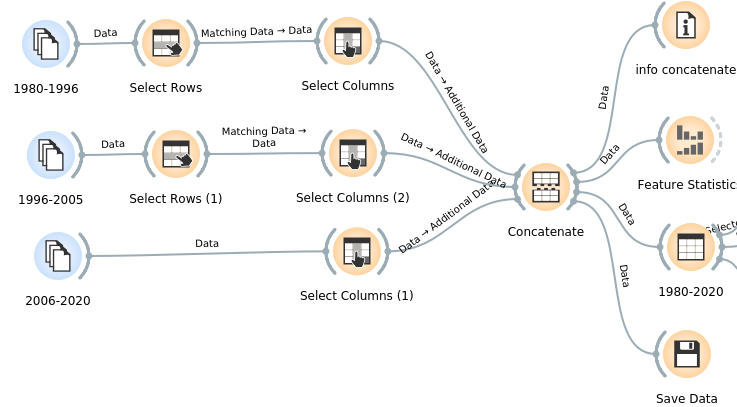
\includegraphics[scale = 0.5]{imagenes/orange1.png}
            \caption{Concatenación de archivos}
            \label{concatenacion}
            \end{figure}
            \begin{figure}
                \centering
                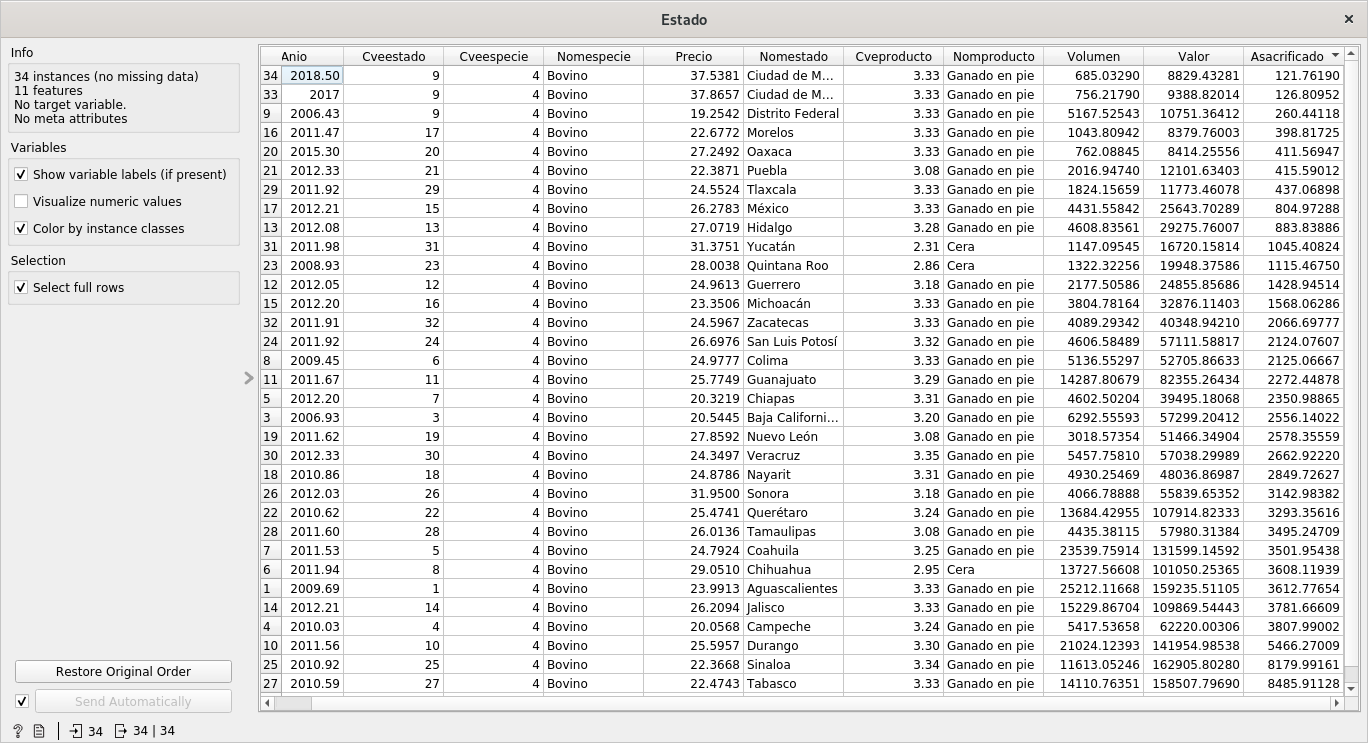
\includegraphics[scale = 0.3]{imagenes/estadosporasacrificado.png}
                \caption{Estados Federativos ordenados por Sacrificados}
                \label{tablesacrificados}
            \end{figure}
            \begin{figure}
                \centering
                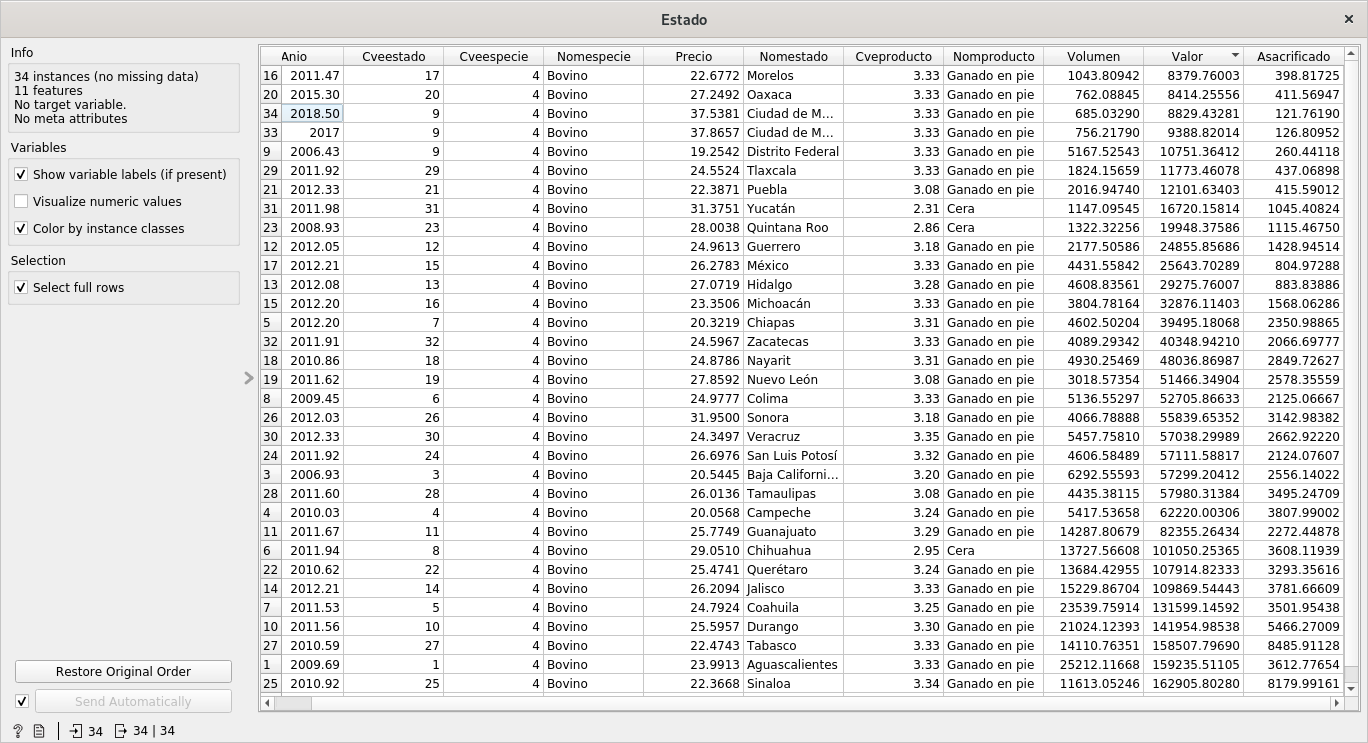
\includegraphics[scale = 0.3]{imagenes/estadosporvalor.png}
                \caption{Estados Federativos ordenados por valor}
                \label{tablevalor}
            \end{figure}
            \newpage
            \item Para el objetivo 2 que es: {\bfseries Ordenar las entidades federativas según el valor promedio de su producción pecuaria para cada año el periodo que se estudia para la especie “Bovina”}, hicimos el mismo procedimiento que el anterior, obteniendo claro la siguiente imagen en la figura 3.
            \item En el objetivo 3: \\ {\bfseries Grafique la relación entre los valores para el crecimiento promedio y el valor promedio establecidos en las tareas anteriores para cada una las entidades: Veracruz, Sonora, Tamaulipas, Sinaloa, Oaxaca. ¿Qué observa?}, primero tuvimos que filtrar los estados por medio de {\bfseries Orange} para solo seleccionar los estados que nos pedían. \\
Una vez que tenemos el filtro procedimos a obtener la siguiente gráfica en la cual se ve que: Sinaloa fue el estado con un promedio más alto tanto en producción como en valor, enseguida se adjuntan las imágenes de lo obtenido.\\
Se observa que Sinaloa es el mayor en ambas gráficas.
            \begin{figure}[htb!]
                \begin{minipage}[b]{0.5\linewidth} %Una minipágina que cubre la mitad de la página
                \centering
                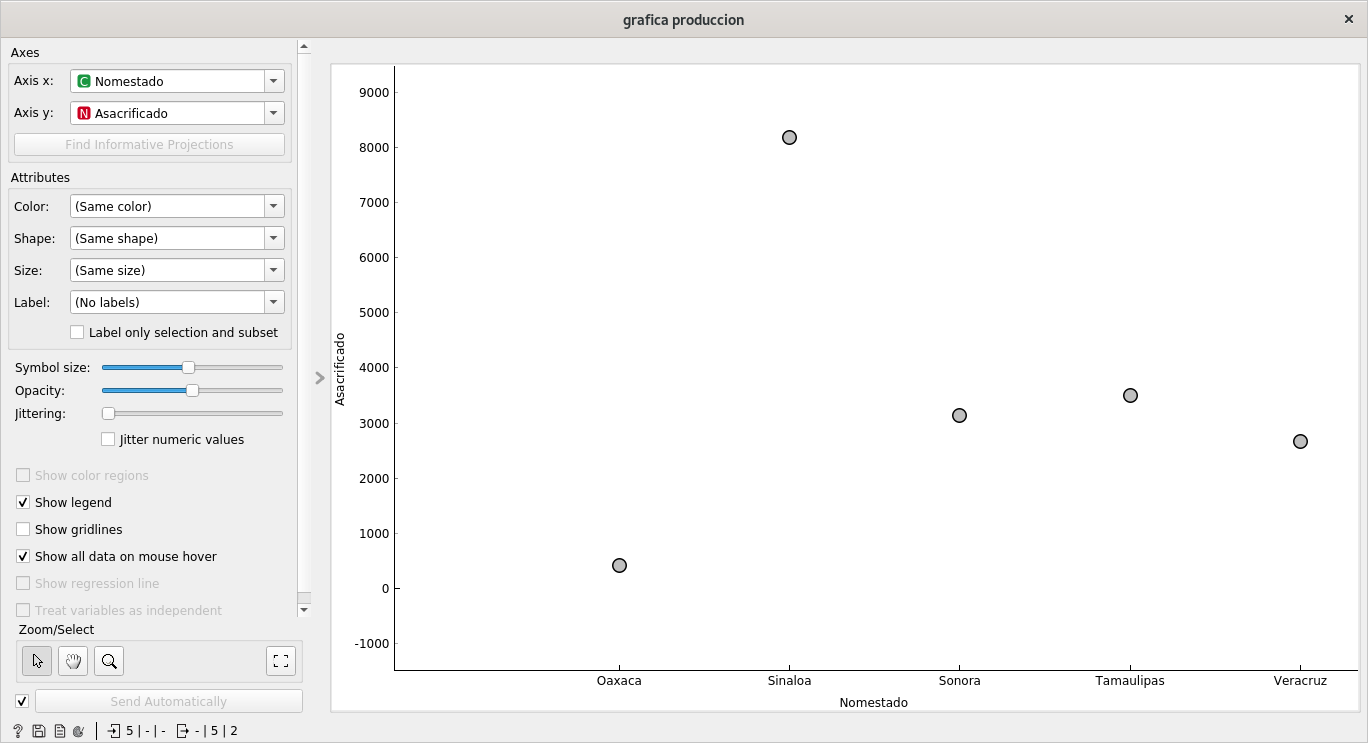
\includegraphics[width = 8cm]{imagenes/graficaestados-sacrificados.png}
                \caption{Gráfica Estados ordenados por sacrificio}
                \label{graficaestadossacrificio}
                \end{minipage}
                \hspace{0.5cm} % Si queremos tener un poco de espacio entre las dos figuras
            \begin{minipage}[b]{0.5\linewidth}
                \centering
                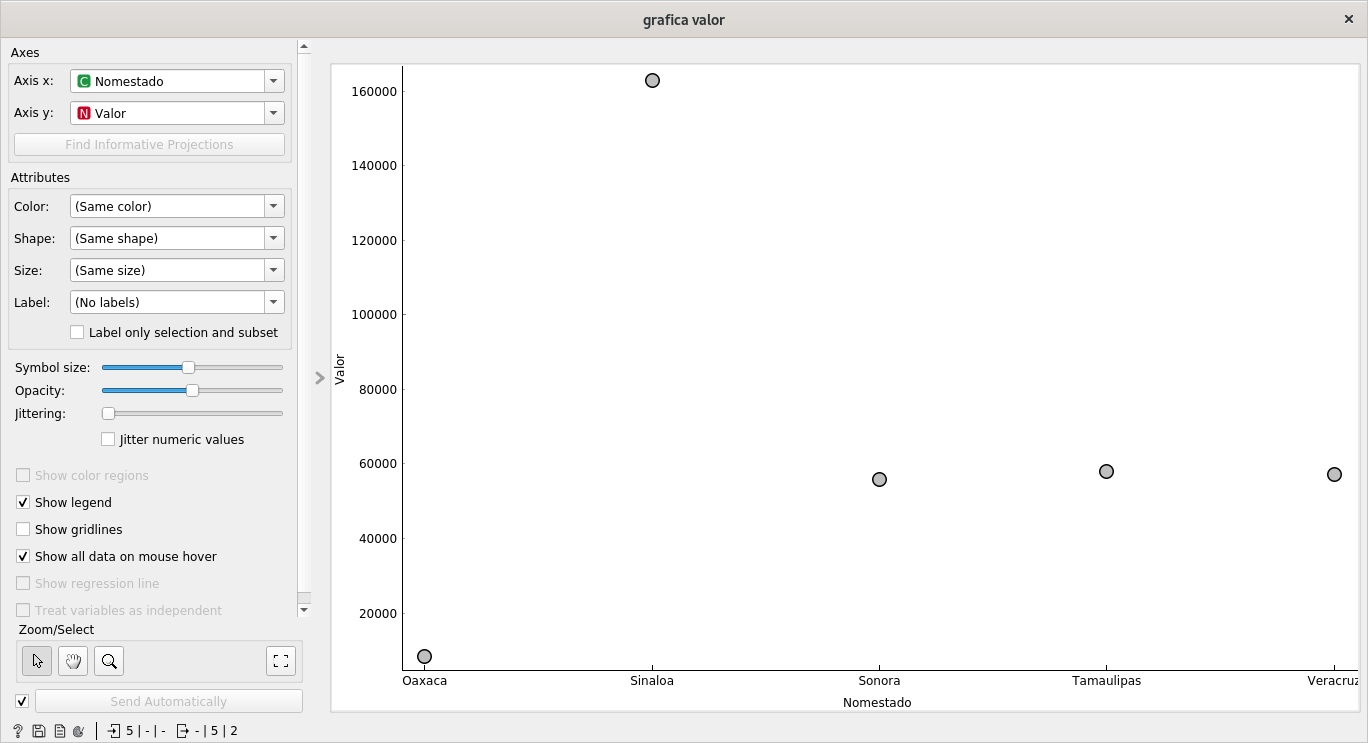
\includegraphics[width = 8 cm ]{imagenes/graficaestados-valor.png}
                \caption{Gráfica Estados ordenados por valor}
                \label{graficaestadosvalor}
                \end{minipage}
            \end{figure}
\newpage
            \newpage
            \item En este objetivo es en el que decidiremos nuestra hipótesis, la cual si recordamos era que no existía ninguna correlación entres los valores de nuestros registros.\\
Una vez que teniamos nuetra tabla filtrada por los datos pedidos en el objetivo anterior pasamos a obtener su coeficientes de correlación de Spearman, los cuales se muestran en la siguiente imagen \\
            \begin{figure}[h]
                \centering
                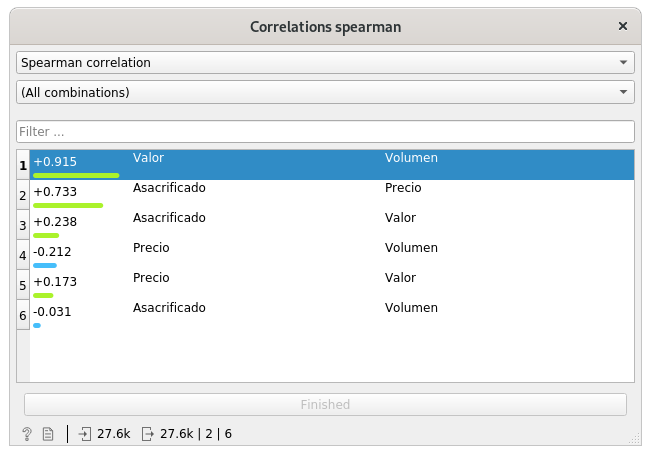
\includegraphics[scale = 0.3]{imagenes/correlacion.png}
                \caption{Correlación de Spearman}
                \label{correlacion}
            \end{figure}
\\Como podemos ver existen varias correlaciones, pero las más importantes son las existentes entre Valor-Volumen y Asacrificado-Precio, por lo cual podemos rechazar nuestra hipótesis.
            
            \item Para este objetivo tuvimos que filtrar de nuevo como se ve en la figura \ref{filtrosnuevos}, ya que solo nos pedían los estados de Veracruz y Tamaulipas y además teniamos que dividir el año 2020; después de esto pasamos a crear un guardado e incorporarlo en el documento, para hacer una predicción como se muestra en la figura \ref{tercerfiltro}, de igual manera cargamos los datos reales y los graficamos enseguida se adjuntan ambas imágenes.
\begin{figure}[h]
    \centering
    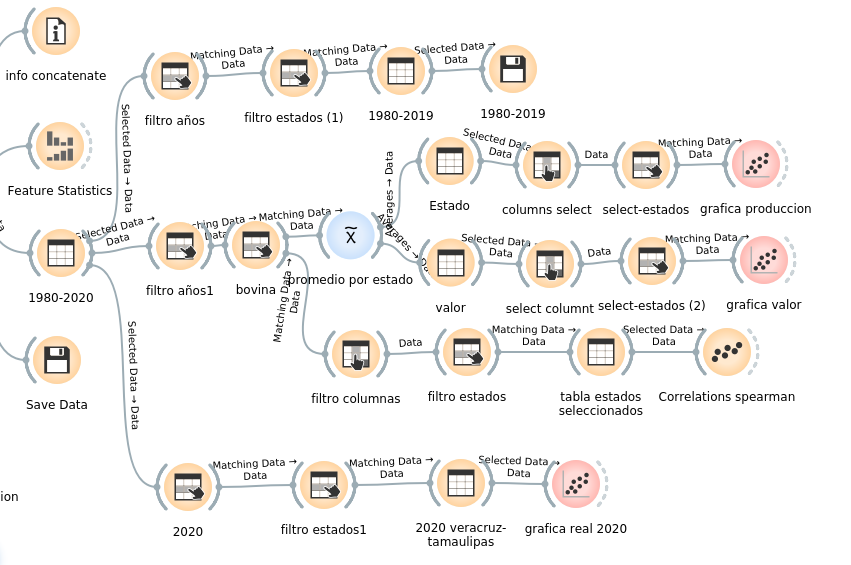
\includegraphics[scale = 0.4]{imagenes/Orange2.png}
    \caption{Filtros Nuevos}
    \label{filtrosnuevos}
\end{figure}
\begin{figure}[h]
    \centering
    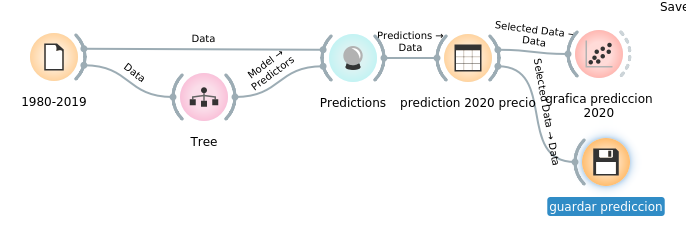
\includegraphics[scale = 0.5]{imagenes/orange3.png}
    \caption{Tercer filtro}
    \label{tercerfiltro}
\end{figure}
\begin{figure}[htb!]
\begin{minipage}[b]{0.5\linewidth} %Una minipágina que cubre la mitad de la página
\centering
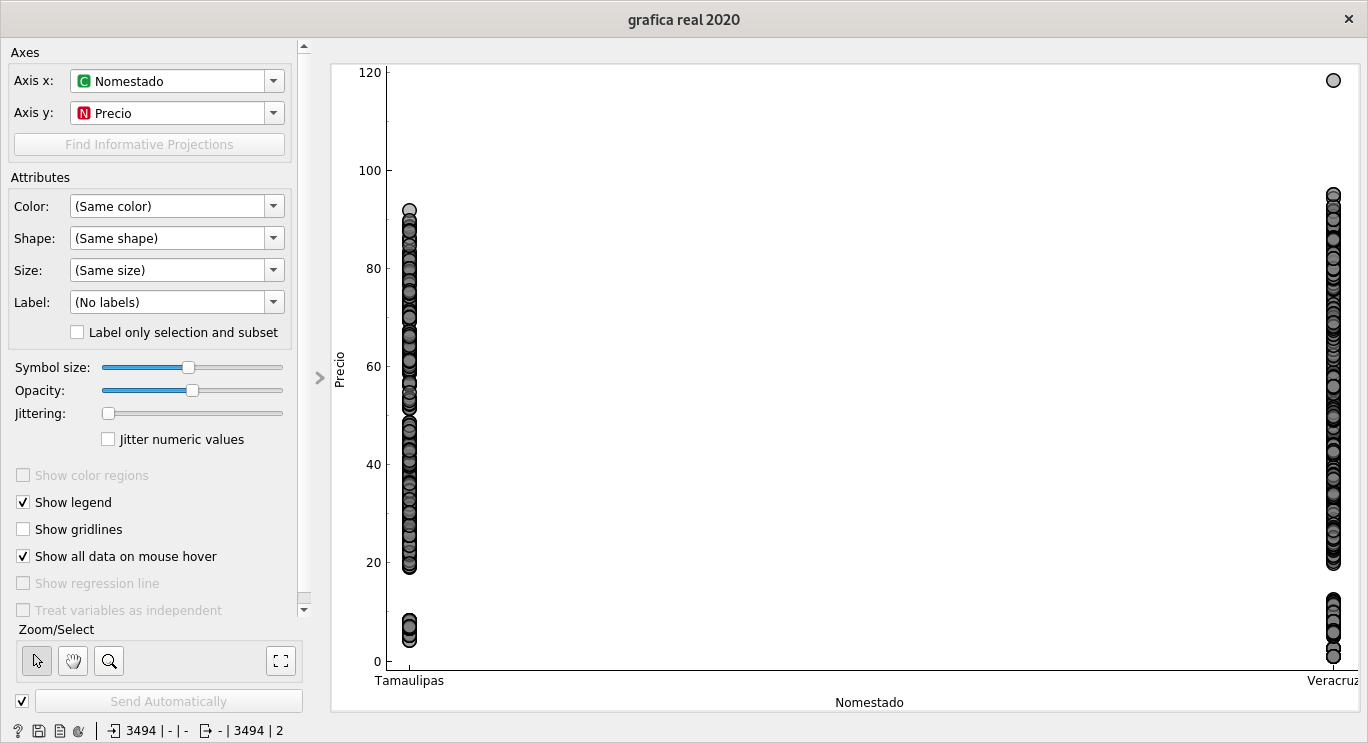
\includegraphics[width=8cm]{imagenes/grafica-real-2020.png}
    \caption{Gráfica real 2020}
    \label{graficareal}
\end{minipage}
\hspace{0.5cm} % Si queremos tener un poco de espacio entre las dos figuras
\begin{minipage}[b]{0.5\linewidth}
\centering
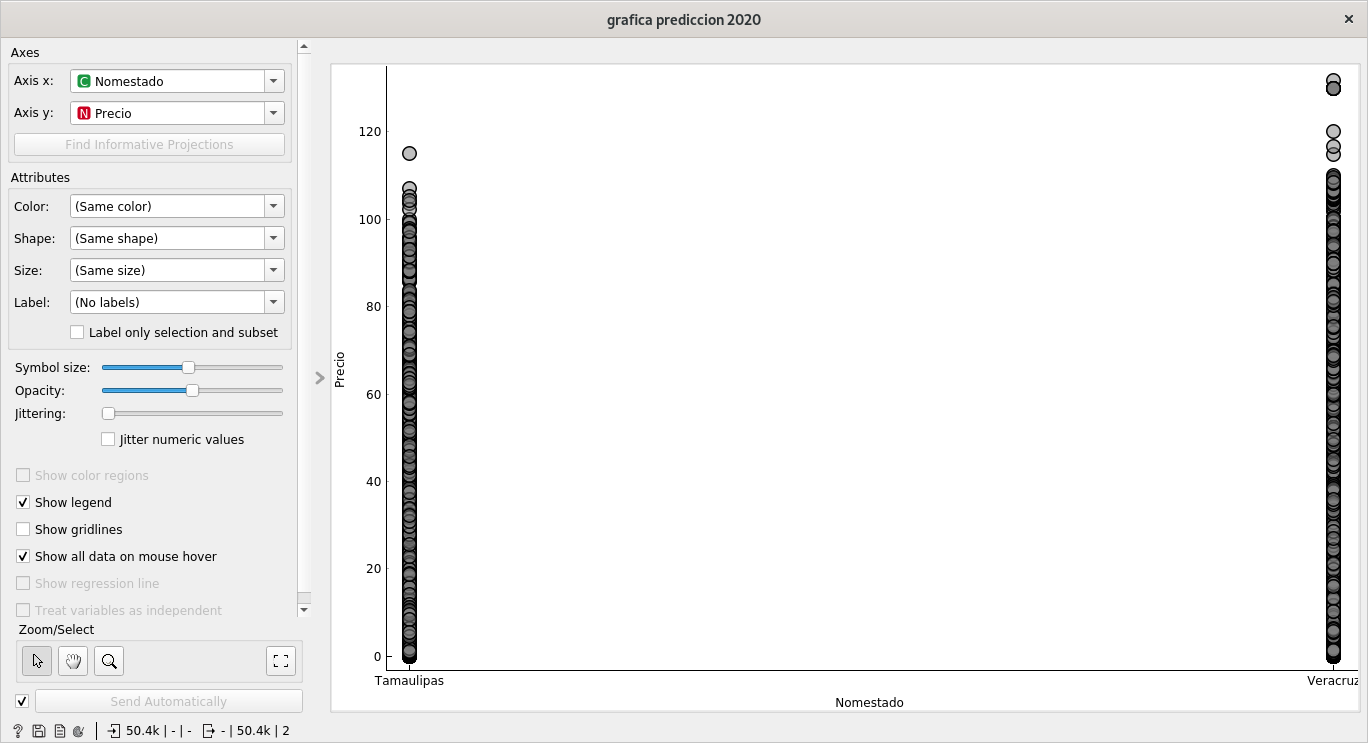
\includegraphics[width=8cm]{imagenes/grafica-prediccion.png}
    \caption{Gráfica predicción 2020}
    \label{graficaprediccion}
\end{minipage}
\end{figure}
\newpage
Como podemos ver la gráfica entre ambas es demasiado similar.
Entonces de cierto modo podemos decir que nuestra predicción es demasiado cerca a los datos reales.
        \end{enumerate}


\end{enumerate}

\newpage
\subsection*{Diagrama}
El diagrama se modificó demasiadas veces, pero finalmente llegamos a esto:
\begin{figure}[htb!]
    \centering
    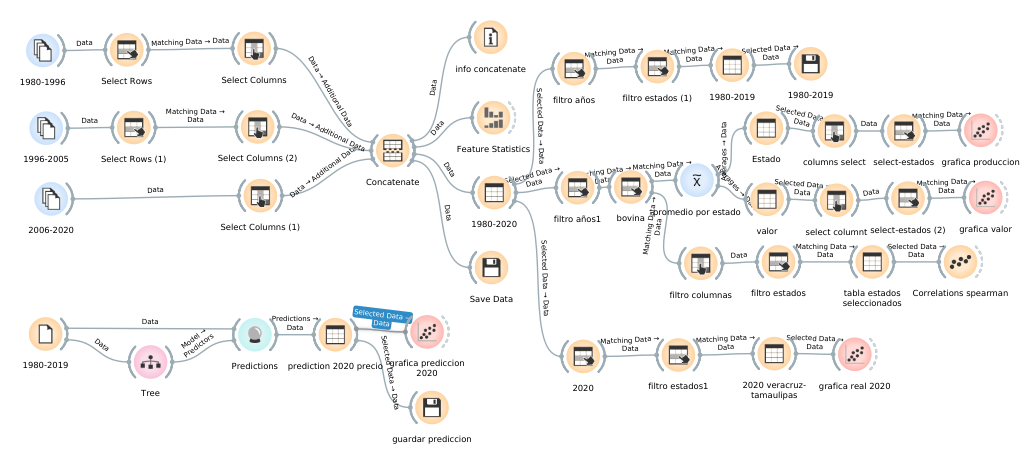
\includegraphics[width = 17 cm]{imagenes/diagrama.png}
    \caption{Diagrama final.}
    \label{diagrama}
\end{figure}

 Llegamos a este diagrama después de varios intentos, obtamos por crear varias ramificaciones ya que se facilitaba visualizar las gráficas sin necesidad de mover los filtros o los ejes.    
\newpage

\section*{Resultados}
Los resultados que obtuvimos son los siguientes:
\begin{enumerate}[I.]
    \item De las gráficas obtenidas al ordenar las entidades federativas, observamos que Sinaloa tiene un crecimiento demasiado desproporcionado a las demás.
    \item Observando las correlaciones que obtuvimos podemos observar que el volumen y valor están muy relacionados entre sí, así como el número de sacrificados y su precio. \newpage 
    \item Y por último la predicción que hicimos del año, si bien no es la misma, podemos observar que están en el mismo rango de valores y son casi idénticos en este último.
\begin{figure}[!h]
    \centering
    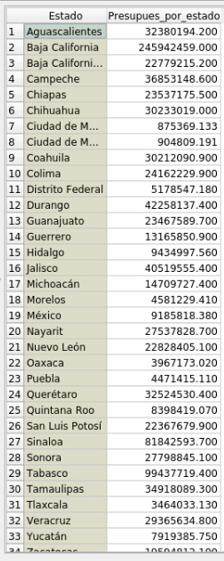
\includegraphics[width = 6 cm]{prep.jpeg}
    \caption{Presupuesto por estado}
    \label{diagrama}
\end{figure}
\newline
De la tabla que fue mostrada podemos ver cuál es la propuesta de presupuesto para cada uno de los estados. Y otra manera de visualizarlo es con un gráfico de barras: 
\begin{figure}[h]
    \centering
    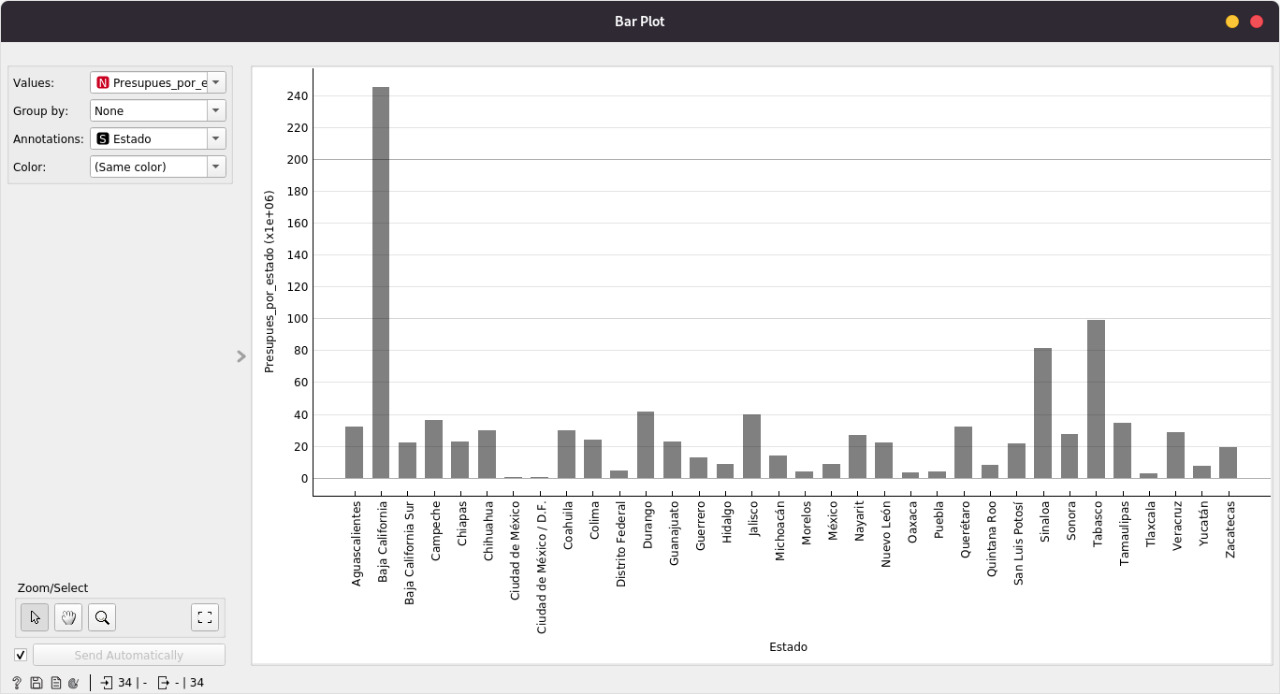
\includegraphics[width = 12 cm]{imagenes/grafica.jpeg}
    \caption{Grafico de barras de presupuesto por estado.}
    \label{diagrama}
\end{figure}


\end{enumerate}

\newpage

\section*{Discusión}
La discusión sería: \\ ¿Qué podemos hacer para decidir si nuestra predicción es realmente eficaz? \\
Se nos ocurrió que tal vez en un futuro, podiamos hacer un análisis entre los valores reales y los valores de la predicción, que por falta de tiempo no pudimos realizar.
¿Realmente es suficiente el análisis de correlación para determinar una estrecha dependencia de las variables? \\
Siguiendo este análisis es casi a simple vista la relación que existe e inclusive podemos decir que es una relación que se esperaba.



\newpage
\newpage
\section*{Conclusión}
En primer lugar que una buena predicción sobre cuanto es necesario producir para tratar de estar lo más apegado a la demanda estimada del próximo año es evitar desperdicios de recursos y capital, y que la economía no sea alterada para mal por este tipo de errores. \\
Por otro lado, al comparar la producción REAL de las entidades federativas de Varacruz y Tamaulipas con respecto a lo que nosotros obtuvimos por medio de nuestro análisis estadístico observamos que fueron muy similares por lo que concluimos que hay consistencia de lo producido este año con respecto a los años pasados. 









\end{document}
